\documentclass{article}
\usepackage{amsfonts, amsmath, amssymb, amsthm, dsfont} % Math notations imported
\usepackage{enumitem}
\usepackage{graphicx}
\usepackage{setspace}
\usepackage{indentfirst}
\usepackage[margin=1in]{geometry}
\graphicspath{{./images/}} % Path to images

% \begin{figure}[htb!]
%      \centering
%      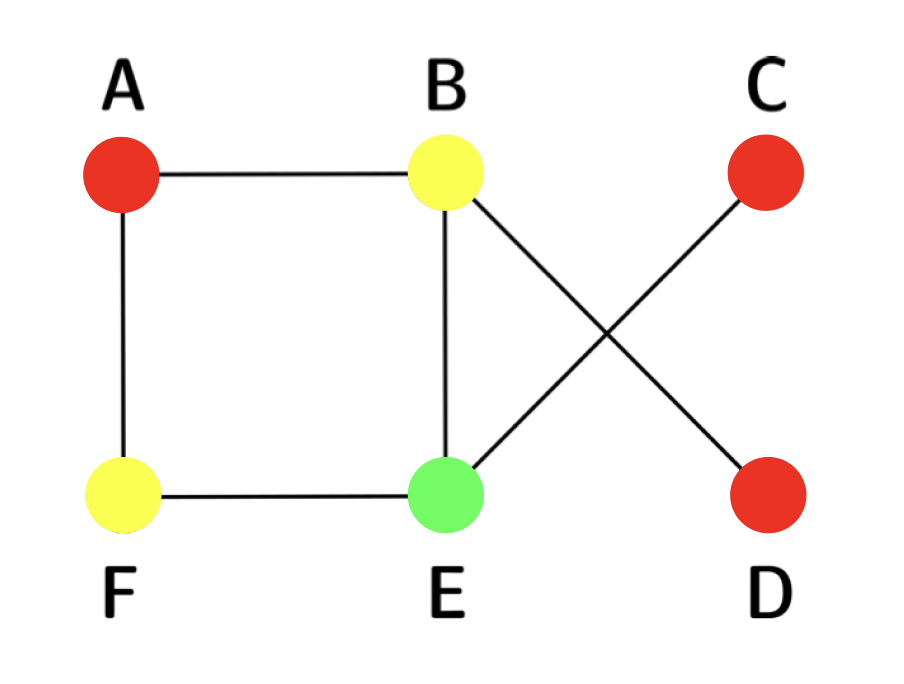
\includegraphics[scale=0.5]{coloring.png}
%      \caption{Coloring of the graph.}
% \end{figure}

% \begin{figure}[htb]
%     \qquad
%     \begin{minipage}{.4\textwidth}
%         \centering
%         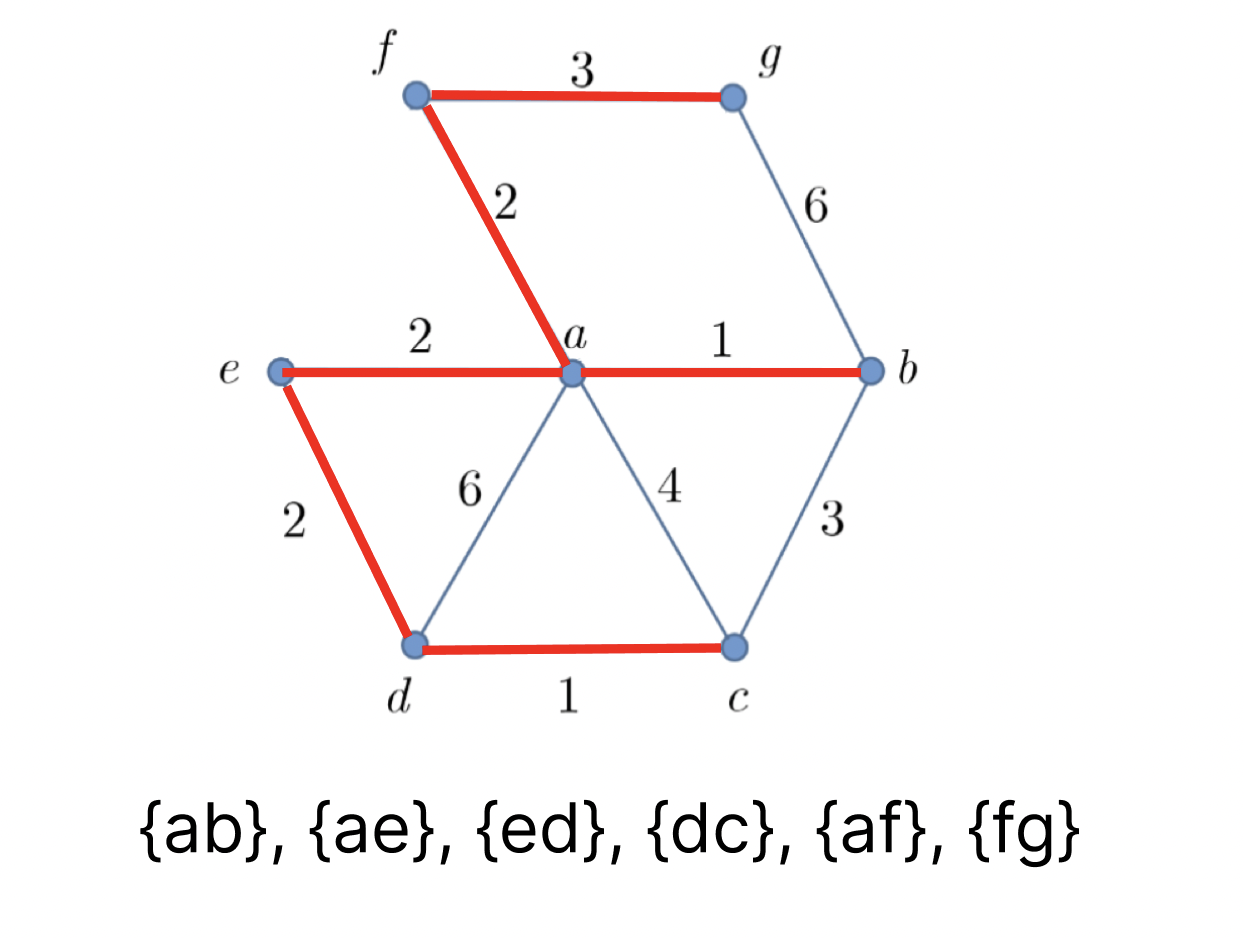
\includegraphics[scale=0.35]{prims.png}
%         \caption{}
%     \end{minipage}    
%     \qquad
%     \begin{minipage}{.4\textwidth}
%         \centering
%         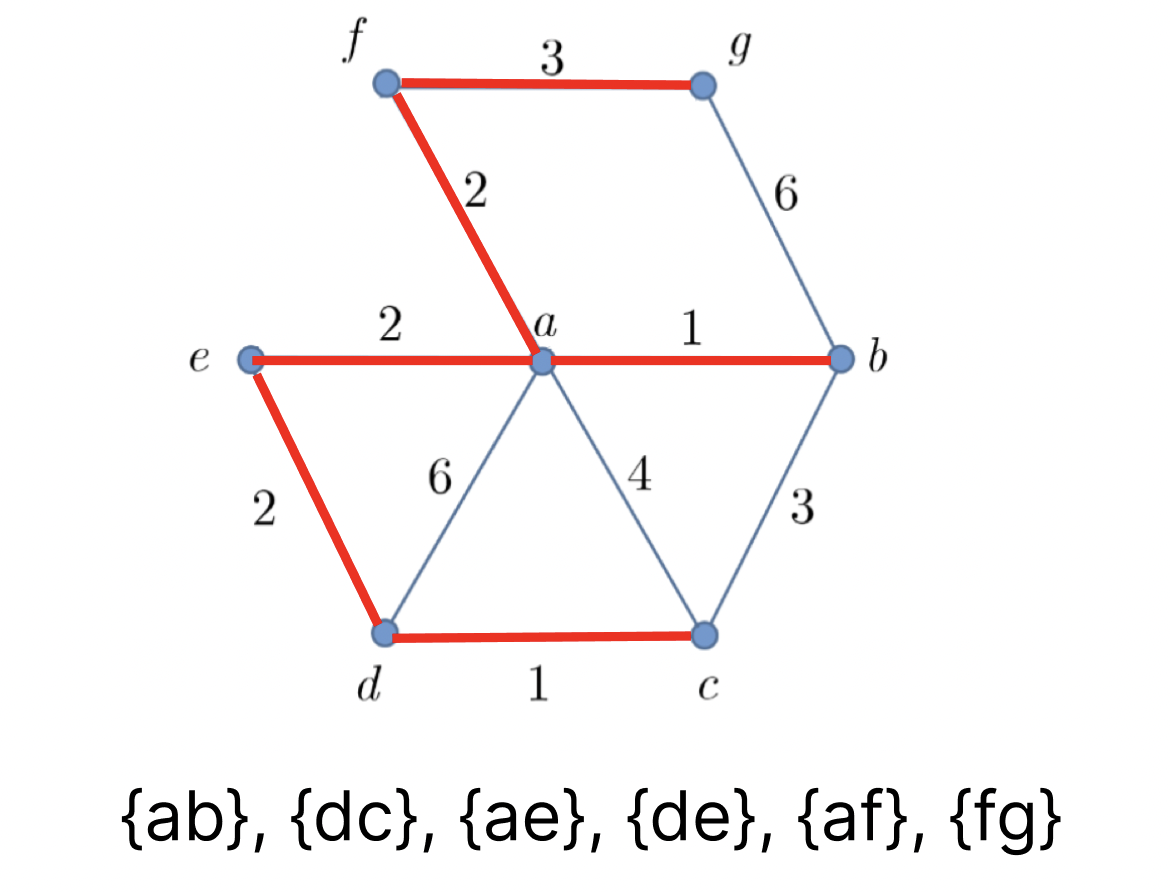
\includegraphics[scale=0.35]{kruskal.png}
%         \caption{}
%     \end{minipage}        
% \end{figure} 

\newtheorem{thm}{Theorem}
\newtheorem{proposition}[thm]{Proposition}
\newtheorem{corollary}[thm]{Corollary}
\newtheorem{lemma}[thm]{Lemma}

\newcommand*{\Var}{\ensuremath{\mathrm{Var}}}
\newcommand*{\Cov}{\ensuremath{\mathrm{Cov}}}
\newcommand*{\Corr}{\ensuremath{\mathrm{Corr}}}
\newcommand*{\Bias}{\ensuremath{\mathrm{Bias}}}
\newcommand*{\MSE}{\ensuremath{\mathrm{MSE}}}
\newcommand*{\range}{\ensuremath{\mathrm{range}}\,}
\newcommand*{\spann}{\ensuremath{\mathrm{span}}\,}
\newcommand*{\nul}{\ensuremath{\mathrm{null}}\,}
\newcommand*{\dom}{\ensuremath{\mathrm{dom}}\,}
\renewcommand*{\implies}{\ensuremath{\Longrightarrow}}
\renewcommand*{\impliedby}{\ensuremath{\Longleftarrow}}
\newcommand*{\Z}{\ensuremath{\mathbb{Z}}}
\newcommand*{\Q}{\ensuremath{\mathbb{Q}}}
\newcommand*{\R}{\ensuremath{\mathbb{R}}}
\newcommand*{\F}{\ensuremath{\mathbb{F}}}
\newcommand*{\C}{\ensuremath{\mathbb{C}}}
\newcommand*{\N}{\ensuremath{\mathbb{N}}}
\newcommand*{\E}{\ensuremath{\mathds{E}}}
\renewcommand*{\P}{\ensuremath{\mathds{P}}}
\newcommand*{\p}{\ensuremath{\mathcal{P}}}

% title information
\title{Math 104 HW9}
\author{Neo Lee}
\date{11/10/2023}

\setstretch{1.15}
% main content
\begin{document} 

% placing title information; comment out if using fancyhdr
\maketitle 

\subsection*{Exercise 23.1 (a, b, c)}
Find the radius of convergence and determine the exact interval of convergence for
\begin{enumerate}[label=\textbf{(\alph*)}]
    \item $\sum n^2x^n$
    \item $\sum \left(\frac{x}{n}\right)^n$
    \item $\sum\left(\frac{2^n}{n^2}\right)x^n$
\end{enumerate}
\begin{proof}[Solution]\indent
    \begin{enumerate}[label=\textbf{(\alph*)}]
        \item \begin{align*}
            \lim \left|\frac{(n+1)^2}{n^2}\right| & = \lim \left|\frac{n^2+2n+1}{n^2}\right|
            = \lim \left|1+\frac{2}{n}+\frac{1}{n^2}\right| = 1 \\
            \implies \beta & = \lim \sup |x^2|^{\frac{1}{n}} = 1 \\
            \implies R & = \frac{1}{\beta} = 1.
        \end{align*}
        For both $x=1$ and $x=-1$, the series diverges because for $x=1$, $\lim n^2 x^n = \infty$
        and for $x=-1$, the limit does not exist. Hence, the convergence interval is $(-1, 1)$.

        \item 
        \begin{align*}
            & \sum \left(\frac{x}{n}\right)^n = \sum \frac{1}{n^n}x^n \\
            \implies & \beta = \lim \sup \left|\frac{1}{n^n}\right|^{\frac{1}{n}} = 
            \lim \sup \frac{1}{n} = 0 \\
            \implies & R = \infty.
        \end{align*}
        Hence, the series converges for all $x\in\R$.

        \item \begin{align*}
            \lim \left|\frac{2^{n+1}}{(n+1)^2}\cdot\frac{n^2}{2^n}\right| & = 
            \lim \left|\frac{2}{\left(1+\frac{1}{n}\right)^2}\right| = 2 \\
            \implies \beta & = \lim \sup \left|\frac{2^n}{n^2}\right|^{\frac{1}{n}} = 
            \lim \left|\frac{2^{n+1}}{(n+1)^2}\cdot\frac{n^2}{2^n}\right| = 2 \\
            \implies R & = \frac{1}{\beta} = \frac{1}{2}.
        \end{align*}
        For $x=\frac{1}{2}$, 
        $$\sum\left(\frac{2^n}{n^2}\right)\frac{1}{2^n} = \sum\frac{1}{n^2},$$
        which we know converges. For $x=-\frac{1}{2}$,
        $$\sum\left(\frac{2^n}{n^2}\right)\left(-\frac{1}{2}\right)^n = \sum\frac{(-1)^n}{n^2},$$
        which we know converges by the alternating series test. Hence, the convergence interval is
        $\left[-\frac{1}{2}, \frac{1}{2}\right]$.
    \end{enumerate}
\end{proof}

\subsection*{Exercise 23.2 (b)}
Find the radius of convergence and determine the exact interval of convergence for
$\sum \frac{1}{n^{\sqrt{n}}}x^n$.
\begin{proof}[Solution]
    \begin{align*}
        \beta & = \lim \sup \left|\frac{1}{n^{\sqrt{n}}}\right|^{\frac{1}{n}} =
        \lim \sup \frac{1}{n^{\frac{1}{\sqrt{n}}}} = 
        \lim \sup \sqrt{\frac{1}{n^{\frac{1}{\sqrt{n}}}}\cdot \frac{1}{n^{\frac{1}{\sqrt{n}}}}} = 
        \lim \sup \sqrt{\frac{1}{n^{1/n}}} = \sqrt{\lim \frac{1}{n^{1/n}}} = 1 \\
        \implies R & = \frac{1}{\beta} = 1.
    \end{align*}
    For $x=1$, $$\frac{1}{n^{\sqrt{n}}}\le \frac{1}{n^2}\qquad \text{for }n\ge 4,$$
    then by Comparision Test with $\sum \frac{1}{n^2}$, the series converges. For $x=-1$,
    the series converges by the Alternating Series Test. Hence, the convergence interval is
    $[-1, 1]$.
\end{proof}


\newpage
\subsection*{Exercise 23.8}
\begin{proposition}
    For each $n\in\N$, let $f_n(x)=\frac{1}{n}\sin nx$, where each $f_n$ is a differentiable function,
    then 
    \begin{enumerate}[label=\textbf{(\alph*)}]
        \item $\lim f_n(x)=0$ for all $x\in\R$,
        \item but $\lim f'_n(x)$ need not exist [at $x=\pi$ for instance].
    \end{enumerate}
\end{proposition}
\begin{proof}[Solution]\indent
    \begin{enumerate}[label=\textbf{(\alph*)}]
        \item For all $x\in \R$, $|f_n(x)|\le |\frac{1}{n}|$ because $|\sin nx|\le 1$ for all $n\in\N$.
        Then, taking the same $N$ as for the $\epsilon$-proof of the limit of $\frac{1}{n}$, we have 
        $$|f_n(x)-0|<\epsilon,$$ thus $\lim f_n(x)=0$ for all $x\in\R$.

        \item $$f'_n(x)=\cos nx.$$ Specifically, $f'_n(\pi)=(-1)^n$, which does not have a limit.
    \end{enumerate}
\end{proof}


\newpage
\subsection*{Exercise 24.4}
For $x\in[0,\infty)$, let $f_n(x)=\frac{x^n}{1+x^n},$\begin{enumerate}[label=\textbf{(\alph*)}]
    \item Find $f(x)=\lim f_n(x)$.
    \item Determine whether $f_n\to f$ uniformly on $[0,1]$.
    \item Determine whether $f_n\to f$ uniformly on $[0,\infty)$.
\end{enumerate}
\begin{proof}[Solution]\indent
    \begin{enumerate}[label=\textbf{(\alph*)}]
        \item For $x<1$, $\lim x^n=0$, thus $$\lim f_n(x)=0.$$ For $x=1$, 
        $$\lim f_n(x)=\frac{1}{2}.$$
        For $x>1$, 
        $$\lim f_n(x)=\lim \frac{1}{1/x^n+1} = 1.$$
        Hence, $$f(x)=\begin{cases}
            0 & \text{if }x<1 \\
            \frac{1}{2} & \text{if }x=1 \\
            1 & \text{if }x>1.
        \end{cases}$$

        \item For $x\in[0,1]$, $x^n$ is continuous $\implies 1+ x^n$ is continuous and nonzero 
        $\implies \frac{1}{1+x^n}$ is continuous. Hence, $f_n$ is continuous on $[0,1]$ for 
        all $n\in\N$. However, $f$ is not continuous at $x=1$ because 
        $$\lim_{x\to 1^-}f(x)=0\ne \frac{1}{2}=f(1).$$ Therefore, by \emph{Theorem 24.3},
        $f_n$ does not converge uniformly to $f$ on $[0,1]$.

        \item Similarly, $f_n$ is continuous on $[0,\infty)$ for all $n\in\N$. However,
        $f$ is not continuous at $x=1$ because
        $$\lim_{x\to 1^-}f(x)=0\ne \frac{1}{2}=f(1).$$ Therefore, by \emph{Theorem 24.3},
        $f_n$ does not converge uniformly to $f$ on $[0,\infty)$.

        \textbf{More simply}, if $f_n$ converges uniformly to $f$ on $[0,\infty)$, then
        $f_n$ will converge to $f$ uniformly on $[0,1]$, which we have shown to be false. 
        Hence, $f_n$ does not converge uniformly to $f$ on $[0,\infty)$.
    \end{enumerate}
    
\end{proof}

\newpage
\subsection*{Exercise 24.11}
\begin{proposition}
    Let $f_n(x)=x$ and $g_n(x)=\frac{1}{n}$ for all $x\in\R$. Let $f(x)=x$ and $g(x)=0$ for $x\in\R$,
    then
    \begin{enumerate}[label=\textbf{(\alph*)}]
        \item $f_n\to f$ uniformly on $\R$ and $g_n\to g$ uniformly on $\R$;
        \item The sequence $f_ng_n$ does not converge uniformly to $fg$ on $\R$;
    \end{enumerate}
\end{proposition}
\begin{proof}\indent
    \begin{enumerate}[label=\textbf{(\alph*)}]
        \item 
        For $f_n\to f$, take $N=1$, then for all $n> N$ and $x\in\R$,
        $$|f_n(x)-f(x)|=|x-x|=0<\epsilon.$$
        For $g_n\to g$, take $N=\frac{1}{\epsilon}$, then for all $n> N$ and $x\in\R$,
        $$|g_n(x)-g(x)|=\left|\frac{1}{n}-0\right|=\frac{1}{n}<\epsilon.$$

        \item 
        $$(f_ng_n)=\frac{x}{n}, \qquad fg = 0.$$ 
        We show that there does not exist $N$ such that for $n>N$ and all $x\in\R$, 
        $$\left|\frac{x}{n}-0\right|<1.$$ Simply take $x=2N$, then for $n=N+1$, 
        $$\left|\frac{x}{n}-0\right|=\left|\frac{2N}{N+1}\right|>1.$$
    \end{enumerate}
\end{proof}


\end{document}
